%% If you have any problems using this template, please contact the author: %%
%% Chris Carmona: carmona@stats.ox.ac.uk ; chriscarmona.me %%

\documentclass{beamer}

%load any additional packages

\usepackage[UKenglish]{babel}
\usepackage[utf8]{inputenc} % so we can input characters with accents (e.g. ő)

\usepackage{statsbeamer}

\usepackage{graphicx} % ease graphics management
\graphicspath{{images/}} % define folder with images
\usefonttheme{serif} % change font to allow \textbf{}
\usepackage{charter} % Nicer fonts
\usepackage{amsmath,amsthm,amssymb} % for math equations

\usepackage{natbib} % richer citation
\usepackage{breakcites} % avoid overfull hbox for long cites


%% Information (author, title, etc.) %%
\usepackage{tikz}
\usepackage{animate}

\title[Short Title]{% short title for footer
    Coronal heating problem and binary reconnection
    \vspace{0.5cm}
}

\author{Haseeb Asad}

\institute{
        \textit{Department of Mathematics}\\
        \textit{Durham University}
        \vspace{0.5cm}
}
\date[Venue and Date]{% short date for footer
    
}

%% Content of slides %%
%%%%%%%%%%%%%%%%%%%%
\begin{document}
%%%%%%%%%%%%%%%%%%%%

% Title slide %
{
    \setbeamertemplate{footline}{}
    \setbeamertemplate{headline}{}
    \setbeamercolor{background canvas}{bg=oxfordblue}
    \maketitle
}

%now include the slides
\setbeamercovered{transparent}
%----------------------------%
\section{Coronal Heating Problem}
\begin{frame}
    \frametitle{Coronal heating problem}
    \small
    \begin{itemize}
        \item Solar corona reach temperatures of the order $2 \times 10 \text{K}$ whereas surface of the sun is only about $6000\text{K}$.
        \item Unsolved problem: under what mechanism is the energy transported up to the solar corona and converted into heat within a few solar radii.
        \item Two leading theories:
        \begin{itemize}
            \item Wave propagation in magneto-acoustic waves.
            \item Magnetic reconnection.
        \end{itemize}
    \end{itemize}
\end{frame}
%----------------------------%


%----------------------------%
\section{Magnetic Reconnection and binary model}
\begin{frame}
    \frametitle{Magnetic reconnection}
    \small
    \begin{itemize}
        \item Refers to the phenomenon of changing in the topology of field lines i.e. breaking and reconnecting of field lines with opposite directions.
        \item Non-ideal term in Ohm's law can be written as $\textbf{N} = \textbf{E}+\textbf{v}\times\textbf{B}.$ Evolution of magnetic field is then $$ \frac{\partial \textbf{B}}{\partial t} = \nabla\times (\mathbf{\omega}\times \textbf{B})$$.
        \begin{itemize}
            \item 2D reconnection if $\textbf{N} = \textbf{u}\times\textbf{B} + \nabla\Phi$ but $\textbf{u}$ has a singularity.
            \item 3D reconnection if $\textbf{N} \neq \textbf{u}\times\textbf{B} + \nabla\Phi$.
        \end{itemize}
    \end{itemize}
    \begin{figure}
        \centering
        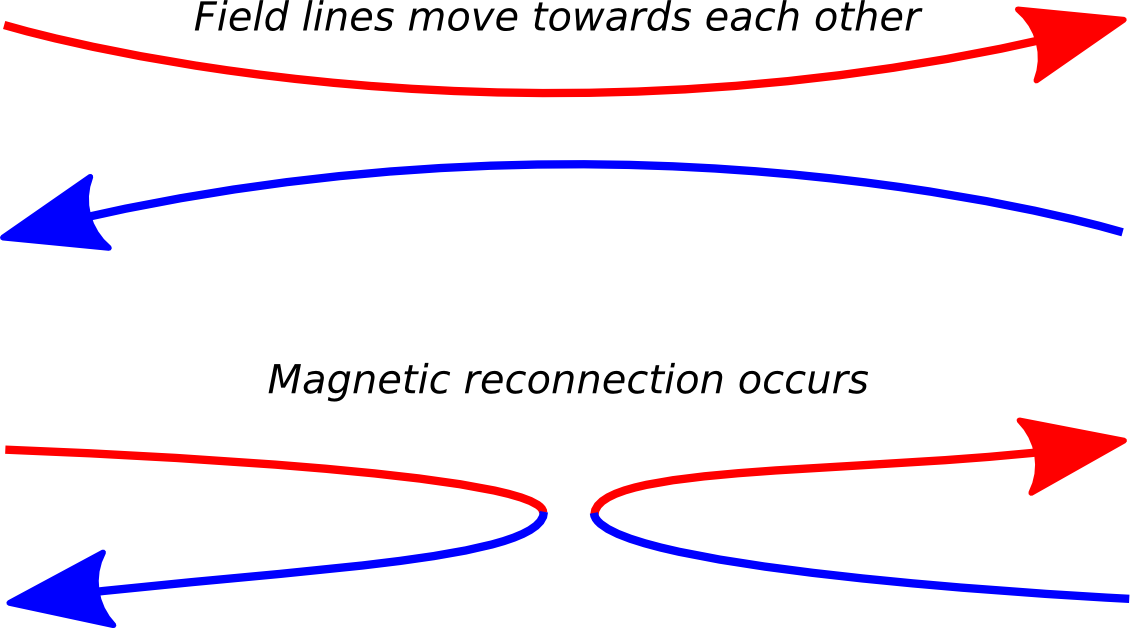
\includegraphics[width=4cm]{images/reconnection.png}
        \caption{Reconnection in magnetic field lines}
        \label{fig:recon}
    \end{figure}
\end{frame}

\begin{frame}
    \frametitle{Helicity}
    \small
    \begin{itemize}
        \item Magnetic helicity of a magnetic vector potential $A$ where $\nabla\times\mathbf{A}=\mathbf{B}$ is defined as 
        \begin{align*}
            H = \int_S \mathbf{A}\cdot\mathbf{B}\, dV.
        \end{align*}
        \item Measures the twisting and linkage of magnetic field lines in a volume.
        \item During reconnection, field lines naturally try to reduce their helicity - untwist themselves.
    \end{itemize}
    \begin{figure}
        \centering
        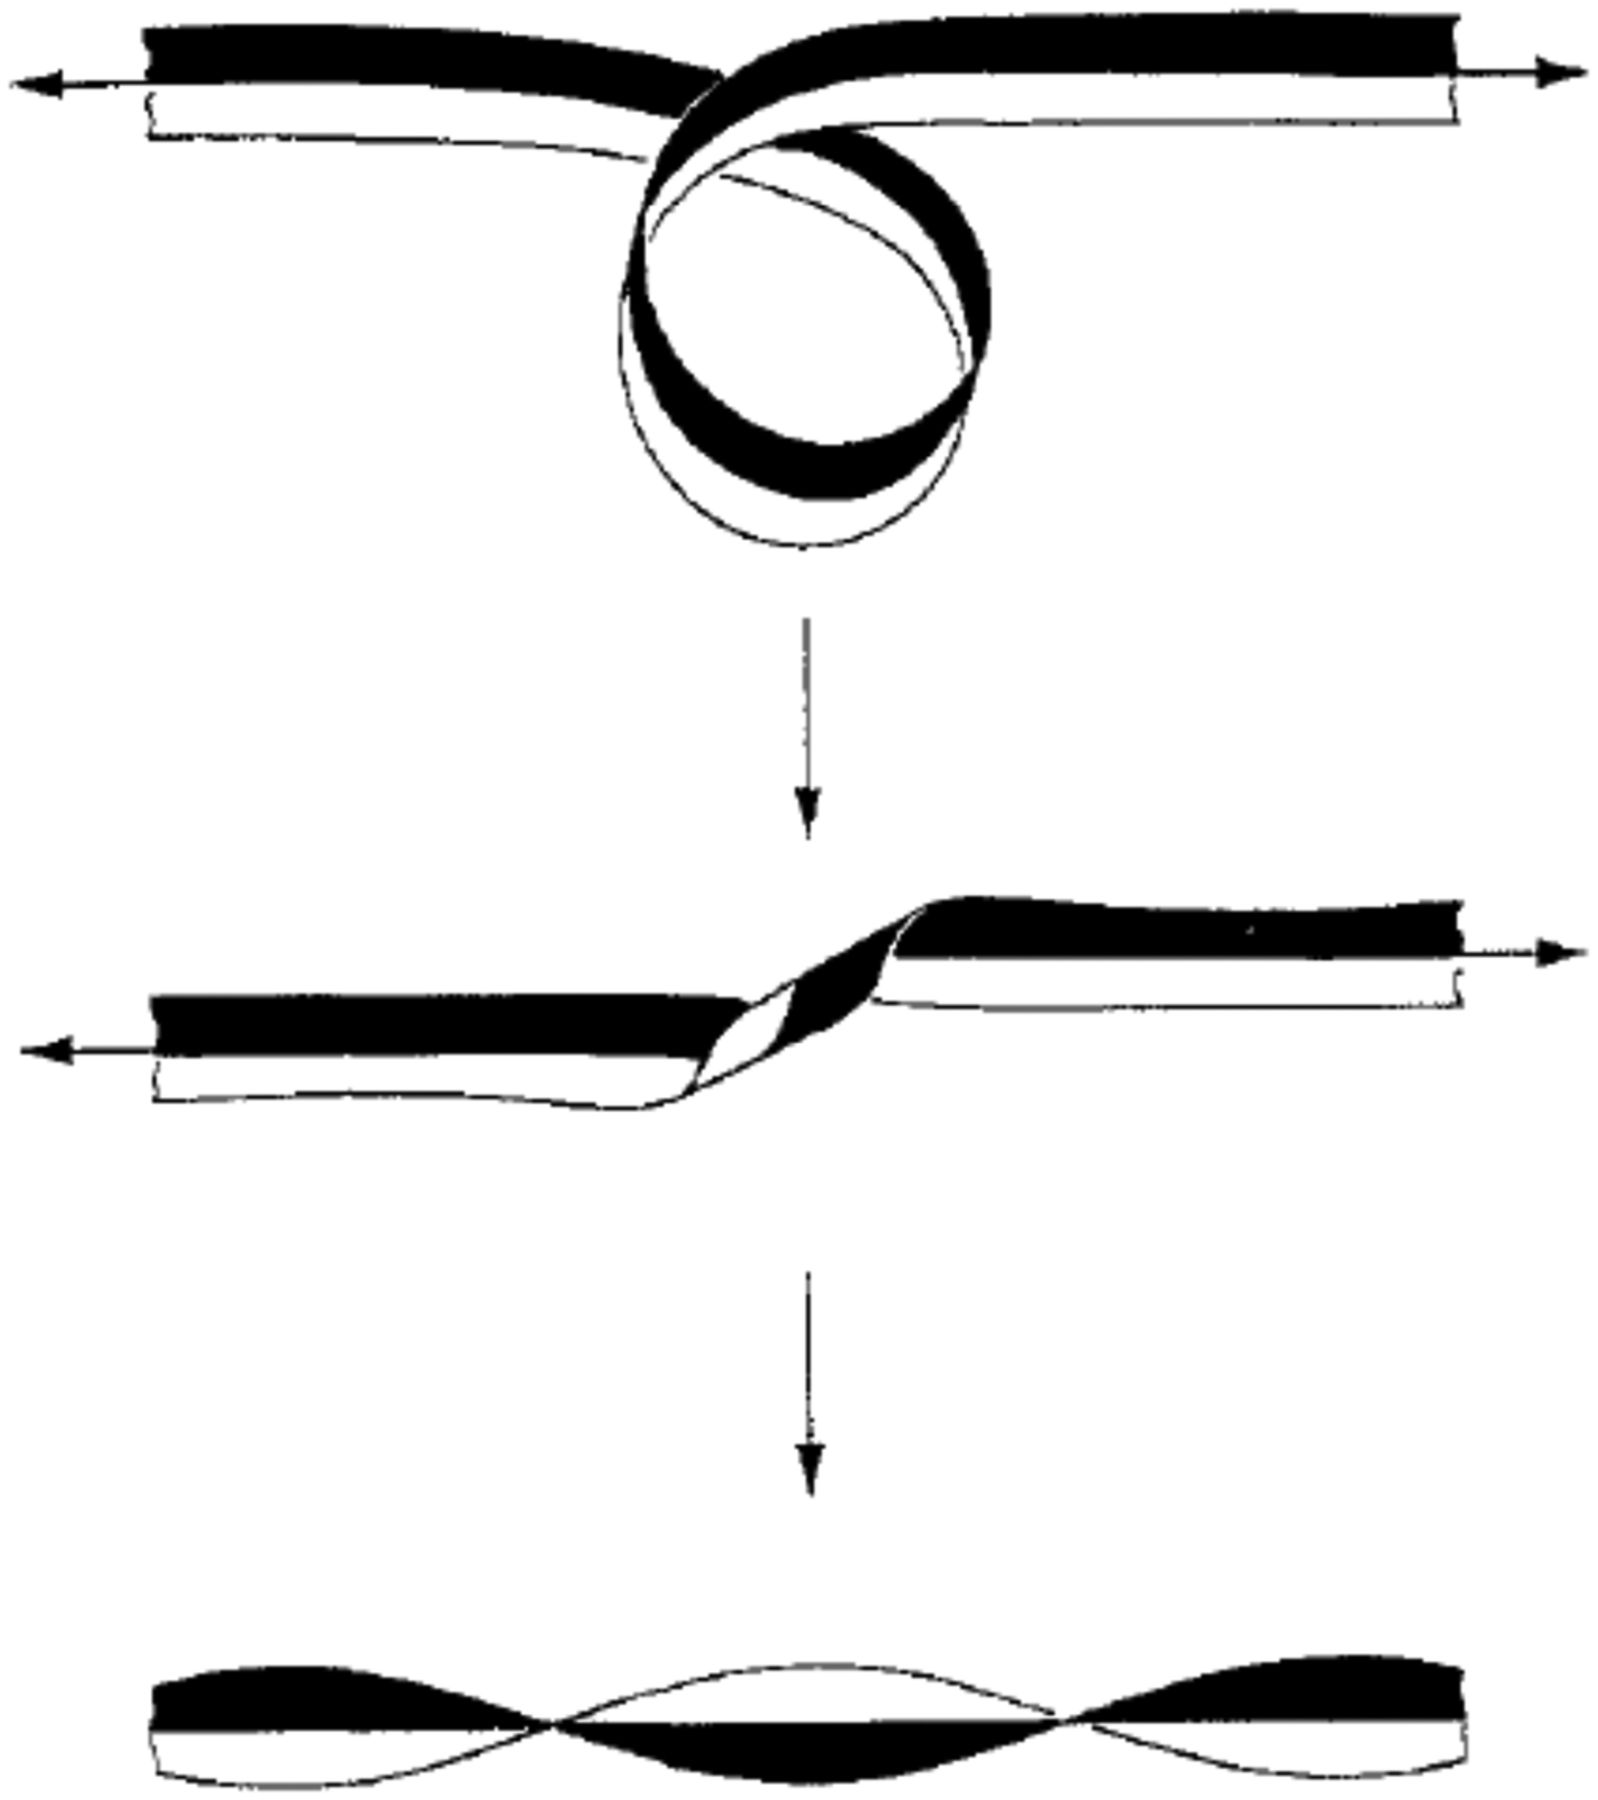
\includegraphics[height=2.75cm]{images/helicity.jpeg}
        \caption{Example of stored helicity and the 'unraveling' of the field line.}
        \label{fig:helicity}
    \end{figure}
\end{frame}
\begin{frame}
    \frametitle{Energy and heating}
    \small
    \begin{itemize}
        \item It is thus this energy stored in the twisted and tangled field lines released in reconnection.
        \item Most of this energy is then converted into thermal energy and heats the solar corona.
        \item Average heating rate due to turbulent reconnection:
        $$Q=\frac{M_T}{2}\sum_{\text{x-line}\,i} l^{+} R_i c_{iAr}B_{ir}^2(\frac{B_{ir}}{B_i})^\gamma.$$ %Be careful of using this without checking.
    \end{itemize}
\end{frame}
%----------------------------%


%----------------------------%
\section{Binary reconnection}
\begin{frame}
    \frametitle{Binary reconnection}
    \small
    \begin{itemize}
        \item Theory proposed by Priest et. al characterised by binary interactions of pair of sources: in the frame of reference of one magnetic element, its corresponding pair may rotate and twist field lines - driving reconnection.
        \item Suggested that more likely to occur in nature given its interactions of the lowest order.
        \item Assumes majority of flux from one source goes to its corresponding sink.
    \end{itemize}
\end{frame}
%----------------------------%


%----------------------------%
\section{Model}
\begin{frame}
    \frametitle{Model}
    \small
    \begin{itemize}
        \item Model magnetic elements as particles following Brownian motion.
        \item Constrained to a box for computation simplicity by implementation of period boundary conditions.
        \item Pick field line starting positions, integrate magnetic field and determine to which particle they end up: approximation of flux between sources.
    \end{itemize}
\end{frame}

\begin{frame}
    \frametitle{Observations}
    \small
    \begin{itemize}
        \item Example model with $N=10$ particles.
        \item Consider the flux distribution of particle 0. 
    \end{itemize}
    \begin{figure}
      \centering
      \begin{tikzpicture}
        \node[anchor=south west,inner sep=0] at (0,0) {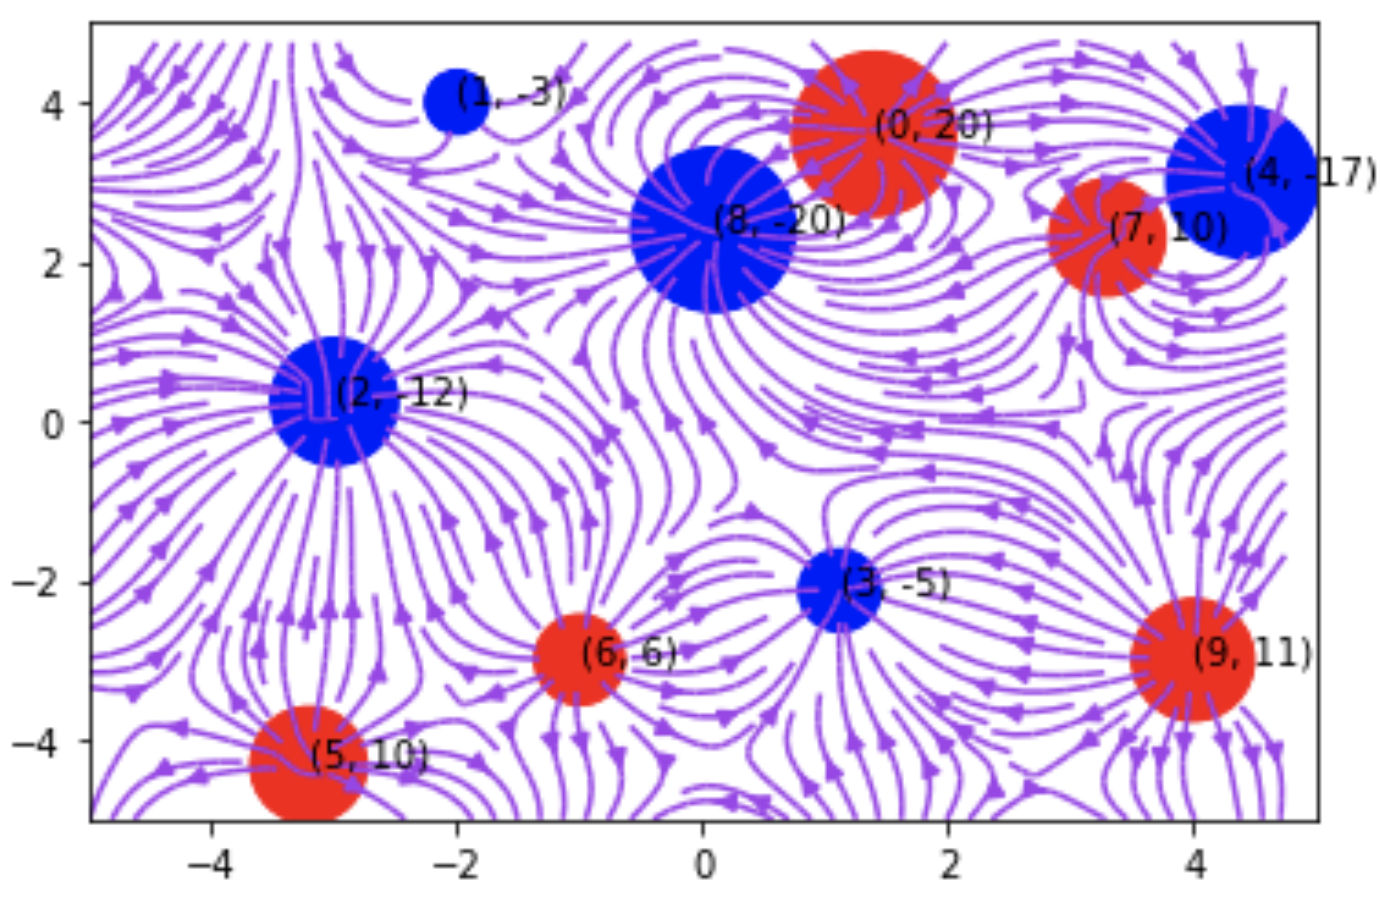
\includegraphics[width=7cm]{images/binary.png}};
        \draw [stealth-, line width = 2pt](4.5,4.1) -- (5.5,5);
        \node[anchor = west] at (5.5,5) {Test particle 0};
      \end{tikzpicture}
      \caption{10 particle model indexed by particle number and magnitude respectively.}
      \label{fig:analysis}
    \end{figure}
\end{frame}
\begin{frame}{Model}
    \small
    \begin{itemize}
    \item Fragments initially appear in opposite polarity, equal magnitude pairs.
    \item As in Meyer's paper, particles may coalesce, break down, end on zero polarity.
    \item Is the model suitable after time evolution? Assumption needs to be tested in late time behaviour.
    \end{itemize}
    \centering
    \animategraphics[loop,width=6cm]{500}{frames/frame}{0}{99}
    
    
\end{frame}
%----------------------------%


%----------------------------%
% Conclusions
\begin{frame}
    \frametitle{}
    \centering
    \Large\color{oxfordblue}
    Thank you!\\
    Haseeb Asad \\
    nsnk94@durham.ac.uk

\end{frame}
%----------------------------%

% References slide
\begin{frame}
\frametitle{References}
\small
\bibliographystyle{apalike} %use the apalike bibliography style
\bibliography{references} % bibliography file
\end{frame}

%%%%%%%%%%%%%%%%%%%%
\end{document}
%%%%%%%%%%%%%%%%%%%%
